% WHERE THIS GOES: paper/sections/08-separation.tex, at the end of the section. It replaces the section's last
% paragraph, which reads exactly:
%   These statements follow from the fields of
%   Sections~\ref{sec:pixel}--\ref{sec:waves}; the estimates of how well each
%   separation works in the presence of noise are still to be made.
% The text below begins with that paragraph's first sentence, kept. With it in place, the item "how well waves can
% be separated from nearby pull in the presence of noise, and the limits of the three-dimensional reconstructions of
% Section~\ref{sec:separation};" of paper/sections/12-status.tex is done, and the promise in the paragraph "How
% precisely" of paper/sections/02b-one-pixel.tex ("it ranges a moving mass with the precision that
% Section~\ref{sec:separation} gives") is kept by Eq.~\eqref{eq:magnetic-range}.
% References: three new entries in paper/drafts/separation_noise.bib (Ross2021, Thompson1982, Reid1990), to be added
% to paper/refs.bib. Figure: paper/figures/separation-noise.pdf, drawn by paper/figures/fig_separation_noise.py.
% Every number: reference/gravcam/separation_noise.py (paper_numbers), checked in
% reference/tests/test_separation_noise.py (test_numbers_quoted_in_the_draft and the tests above it).
% New labels: eq:magnetic-range, eq:depth-bound, fig:separation-noise.

These statements follow from the fields of
Sections~\ref{sec:pixel}--\ref{sec:waves}. How well each works against noise
follows from the Cram\'er--Rao bounds of the same fields, which the reference
implementation computes and checks against fits to simulated noisy readings
(Fig.~\ref{fig:separation-noise}). Each of a pixel's ten numbers carries white
noise, and $\rho$ is the signal-to-noise ratio of a signal at one pixel:
$|\mathcal{W}|/\sigma$ for one reading, as in Section~\ref{sec:one-pixel}, added
in quadrature over a record.

\paragraph{Separation with noise.} Take a wave at $100\,\mathrm{Hz}$ of strain
$10^{-21}$ and, $3\,\mathrm{m}$ from the camera, a rotor of two
$1\,\mathrm{kg}$ masses $12\,\mathrm{cm}$ apart turning 50 times a second,
about the quadrupole of the rotor that calibrates LIGO by its pull
\cite{Ross2021}. Its changing tide has the wave's frequency and a hundred times
its size. Shape alone tells an isolated wave from an isolated mass: the nearest
wave to the field of a mass, and the nearest mass to a wave, lie at half the
reading's size, so one reading of $\tE$ puts the two $\rho/2$ standard
deviations apart, and at $\rho = 12$ fewer than one reading in a hundred is
taken for the other. A wave and a near field together are separated by the
magnetic part, at a fixed price. Let the near field's $\tE$ at the wave's
frequency be anything at all, and its $\tB$ below the noise. Fitting both then
enlarges the error of the wave's amplitude by exactly $\sqrt2$, however strong
the near field: the near field takes the wave's $\tE$, and the wave is read from
its $\tB$, which carries half its signal. The wave is seen at $\rho/\sqrt2$, and
the near field pays the same $\sqrt2$ in the two components it shares with the
wave and nothing in the other three. Ignored, the rotor would be read as a wave
35 times the true one. Its own magnetic part leaks less than $10^{-4}$ of the
wave, because the $\tB$ of a changing source in the near zone is smaller than
its $\tE$ by a factor of order $kr$, here $2\times10^{-6}$, not by $v/c$. An
array that reads only $\tE$ must instead model the rotor from its variation,
here as a point quadrupole of unknown moment and position. For a pixel and six
neighbours at distance $b$ along three axes, the cost $D$, the factor on the
wave's error, grows as $r/b$, because a quadrupole's tide falls as $r^{-5}$ and
its share of the centre's reading must be inferred from a variation smaller by
about $5b/r$. For $b \ll r$, $D$ lies between $0.22\,r/b$ and $0.55\,r/b$ over
orientations. For the rotor and an array one metre across, $b = 0.5\,\mathrm{m}$,
$D = 2.2$; the array overtakes the magnetic part beyond $b = 0.29\,r$, and with
both $D = 1.26$. In return the wave costs the rotor's moment and position
factors of 1.5 and 1.3 from $\tE$ alone, and 1.07 and 1.04 with $\tB$ too.
Modelling the rotor as a point leaves a false wave of $0.005$ of the true one,
from its next multipole, which matters only above $\rho \approx 270$; ignored,
the rotor would be read as 70 times the wave.

\paragraph{How well depth is measured.} For one mass the field and its gradient
give the range exactly, $r = \sqrt{15}\,|\tE|/|\nabla\tE|$ with norms over all
components, and the Cram\'er--Rao bounds on range and mass are
\begin{equation}\label{eq:depth-bound}
\Bigl(\frac{\sigma_r}{r}\Bigr)^2 = \frac{1}{\rho_E^2} + \frac{1}{\rho_G^2},
\qquad
\Bigl(\frac{\sigma_M}{M}\Bigr)^2 = \frac{16}{\rho_E^2} + \frac{9}{\rho_G^2},
\end{equation}
where $\rho_E$ and $\rho_G$ are the signal-to-noise ratios of the field and of
its gradient, whatever the direction. A pixel with six neighbours at distance
$b \ll r$ has $\rho_E = \sqrt7\,\rho$ and $\rho_G = \sqrt{30}\,\rho\,b/r$, so
$\sigma_r/r \approx r/(\sqrt{30}\,\rho b)$; wider, the curvature of the field
across the pixels helps further. For a person $3\,\mathrm{m}$ away and
neighbours $0.5\,\mathrm{m}$ out, $\sigma_r/r$ is between $0.90/\rho$ and
$1.08/\rho$, depending on direction, against $1.16/\rho$ from the closed form
(Fig.~\ref{fig:separation-noise}b). Both uses of the
variation rest on Euler's relation for a field homogeneous of degree $-N$ about
its source, $(\mathbf{x}_s - \mathbf{x})\cdot\nabla f = N f$, with $N = 3$ for
the tide of a mass and $5$ for a quadrupole, by which geophysicists find the
depth of buried sources from measured gradients \cite{Thompson1982,Reid1990}.
The magnetic part of one pixel, Eq.~\eqref{eq:one-pixel-range}, ranges a moving
mass with no neighbours to
\begin{equation}\label{eq:magnetic-range}
\frac{\sigma_r}{r} = \frac{1}{\rho_B} ,
\end{equation}
$\rho_B$ the signal-to-noise ratio of $\tB$ alone, $\sqrt3\,v_\perp/c$ times
that of $\tE$ in each reading: for a person walking at
$1.4\,\mathrm{m\,s^{-1}}$, $\sigma_r/r = 1.2\times10^{8}/\rho$, a hundred
million times worse than with neighbours. Depth along one line is the limit.
For bodies on one line through the pixel every derivative of $\tE$ there has the
pattern of a single mass, so field and gradient see one body at
$r_{\mathrm{eff}} = \sum_i M_i r_i^{-3} / \sum_i M_i r_i^{-4}$, weighted toward
the nearer: two equal masses $\Delta$ apart appear as one at
$r - \Delta^2/r$, and a rod of length $L$ pointing at the camera as a point
$L^2/3r$ nearer than its centre. The spread $s$ of the depths shows first in
the second derivatives, as a share $s^2/r^2$ of them, which the seven pixels
read to $1/\rho_H$, with $\rho_H$ between $8.1$ and $10.5$ times
$\rho\,(b/r)^2$ depending on direction. Two equal masses, $s = \Delta/2$, are
therefore told from one only when $\Delta > 2r/\rho_H^{1/2}$, between $0.62$
and $0.70$ times $(r^2/b)/\rho^{1/2}$: the square-root law that
Section~\ref{sec:near-field} found for masses side by side. A round body of any
size is a point, and its size is not measured at all.

\begin{figure*}
\centering
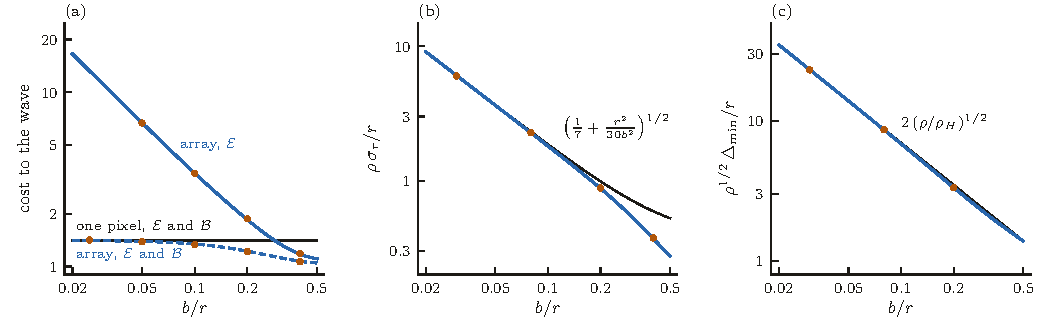
\includegraphics[width=\textwidth]{figures/separation-noise.pdf}
\caption{Separation and depth with noise, against the distance $b$ of a pixel's
six neighbours over the distance $r$ of the source. Blue: Cram\'er--Rao bounds
of the full models; black: closed forms; dots: the spread of
maximum-likelihood fits to simulated noisy readings. (a) The factor $D$ by
which fitting the rotor of the text enlarges the error of a wave's amplitude:
at one pixel from $\tE$ and $\tB$, with any near field, $\sqrt2$ (the dot at
left is a simulation with the rotor present); for the array, which fits the
rotor as a point quadrupole of unknown moment and position, from $\tE$ alone
(solid) and from both (dashed). (b) The range of one mass, with $\rho$ the
signal-to-noise ratio of one pixel's reading, against
Eq.~\eqref{eq:depth-bound}. (c) The separation $\Delta_{\min}$ in depth at which
two equal masses on one line are told from one at one standard deviation.
Computed in the reference implementation.}\label{fig:separation-noise}
\end{figure*}
